\documentclass{article}
\usepackage{amsmath}
\usepackage{amssymb}
\usepackage{amsfonts}
\usepackage[T1]{fontenc}
\usepackage{bm}
\usepackage{array}
\usepackage{graphicx}
\usepackage[utf8]{inputenc}

\title{Paper summary: Curiosity-driven exploration by self-supervised prediction}

\begin{document}
\maketitle


\section{Idea in few sentances}



\section{Explanation of the central concept}




\section{Methodology}


\section{Initial rambly notes}
The paper introduces the intrinsic curiosity module (ICM). It is the paper
that trains a forward prediction model and uses its loss to generate exploration reward (intrinsic reward).
There are problems with it, but it is important to understand because many of the following
methods try to solve the problems this approach has.

\subsection{Abstract}
Curiosity is formulated as the error in the agent's ability to predict
the consequence of its own actions in a visual feature space learned by a self-supervised 
inverse dynamics model.
The method ignores the aspects of the environment that cannot affect the agent, or that the agent
can not affect i suppose.
The paper investigates 3 scenarios:
\begin{enumerate}
		\item sparse extrinsic reward
		\item exploration with no extrinsic reward
		\item generalization to unseen scenarios (or at least faster learning in new scenarios)
\end{enumerate}


\subsection{Introduction}
Other approaches tried to do one of 2 things:
\begin{enumerate}
		\item encourage novelty seeking (exploring unseen states)
		\item encourage the agent to perform actions that reduce the error/uncertainty in the agent's
				ability to predict the consequence of its own actions
\end{enumerate}
The problem with 1) is that a statistical model of the distribution of the environmental states
is required.
2) requires a model that predicts $ (\bm{a}_{t}| \bm{s}_{t} ) \to (\bm{s}_{t+1})  $.
Both of these are hard to do in high-dimensional continuous state spaces such as images.
Also the agent-environment system is inherently stochastic
so the methods fail there.

\subsection{Method}
Reward is:
\begin{equation}
		r_{ t } = r_{ t }^{ i } + r_{ t }^{ e }
\end{equation}
i.e. extrinsic + intrinsic reward, where $ r_{ t }^{ e }  $
will mostly be 0.

The whole architecture can be seen in the following picture:
\begin{figure}[htpb]
		\centering
		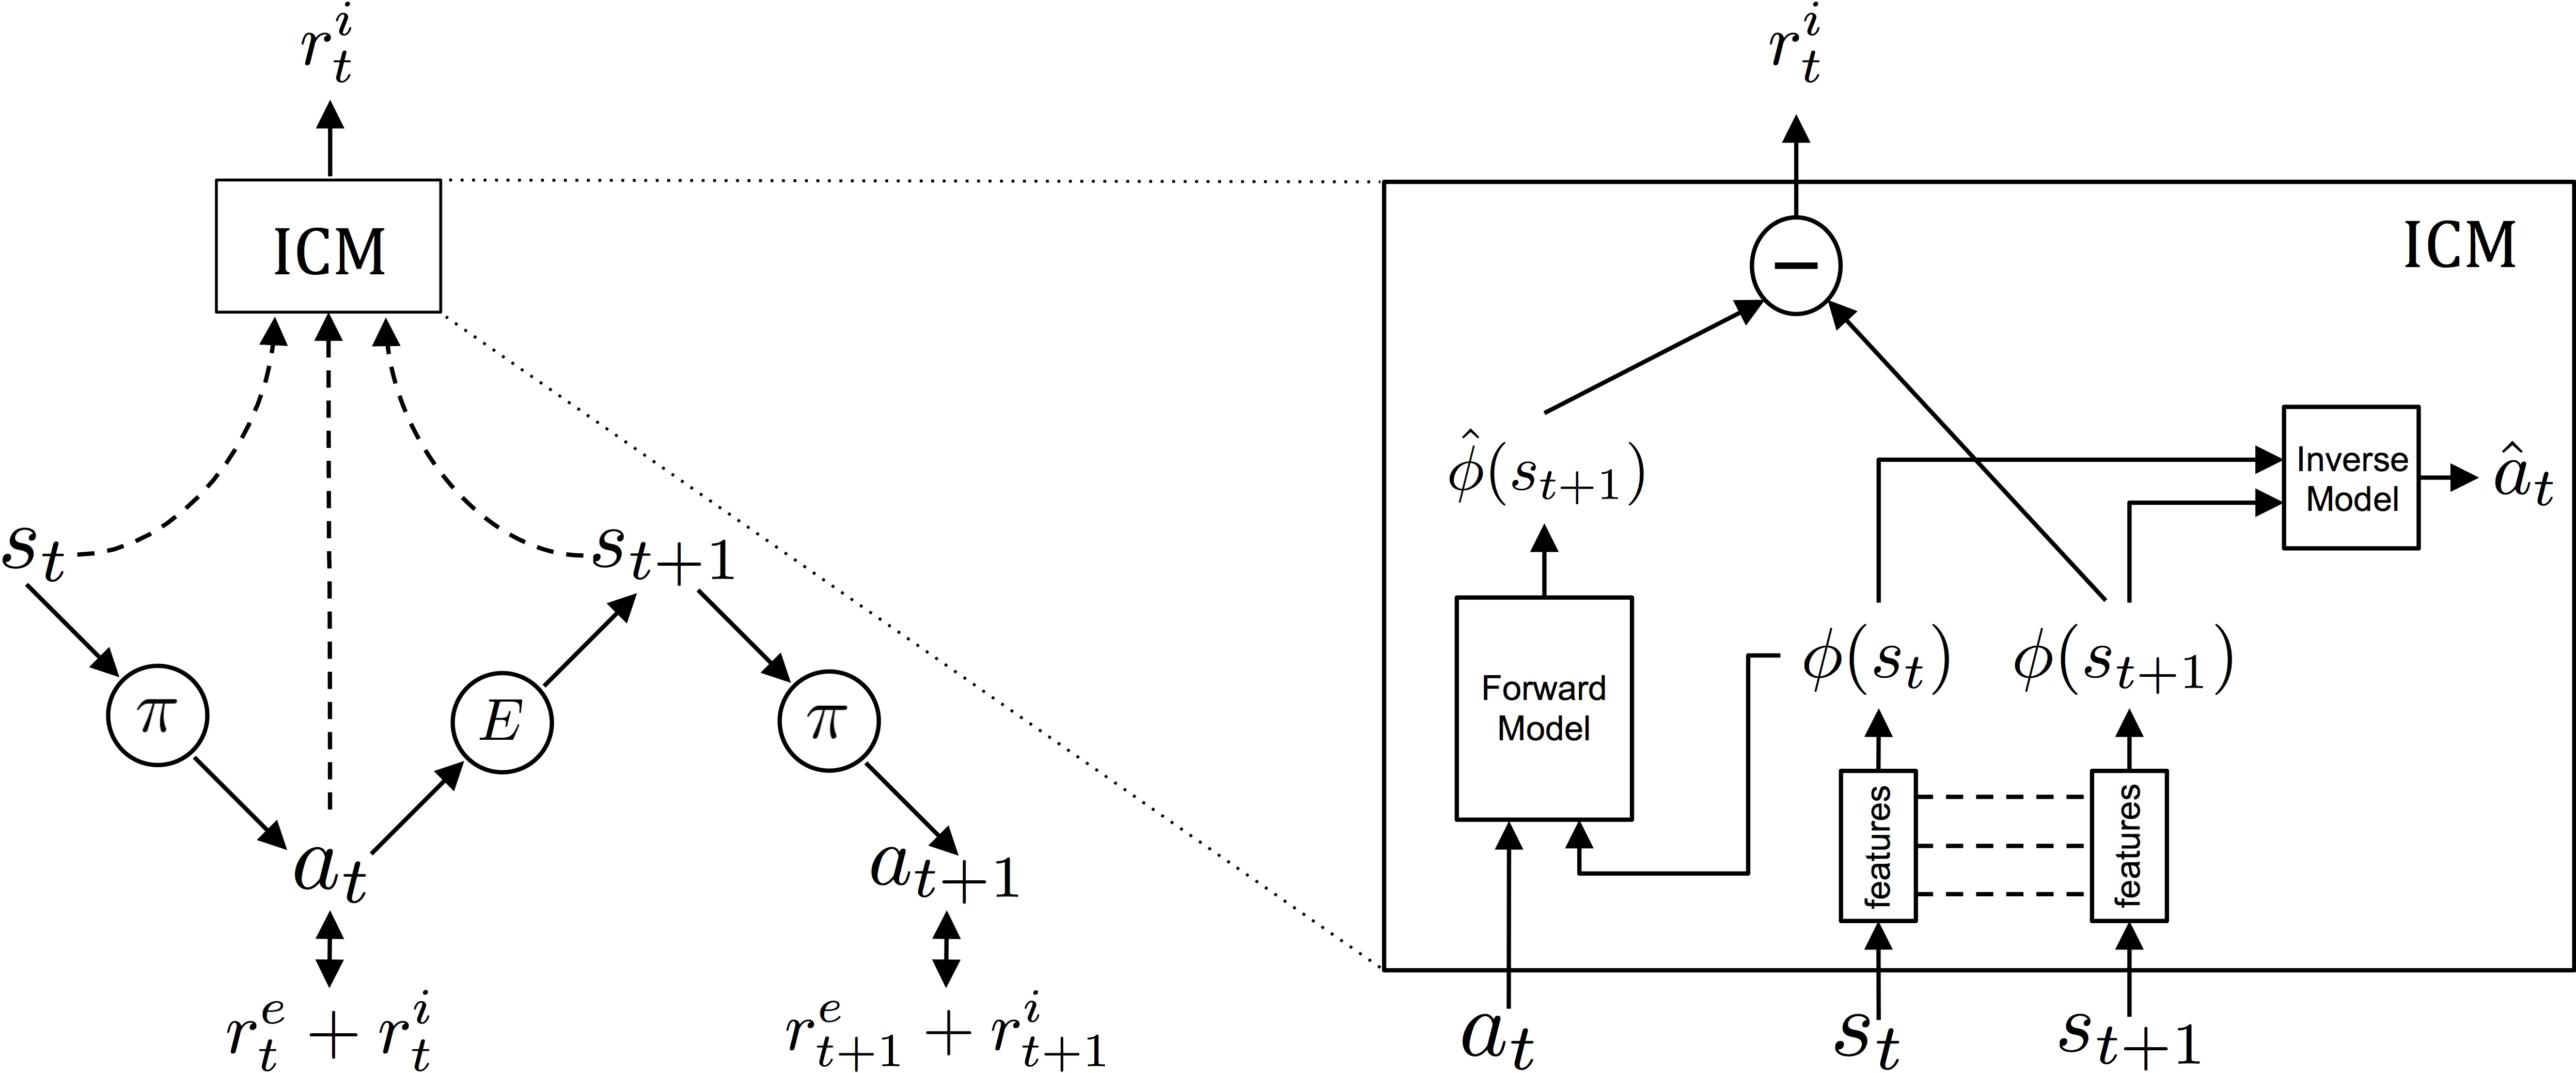
\includegraphics[width=1.0\textwidth]{./method.jpg}
		\caption{Architecture which includes ICM.}
		\label{fig:-method-jpg}
\end{figure}
In words:
\fbox{
\parbox{\textwidth}{
		\ref{fig:-method-jpg}:
		In $ \bm{s}_{t}  $ agent takes $ \bm{a}_{t}  $ sampled from $ \pi  $,
		goes to $ \bm{s}_{t+1}  $.
		$ \pi  $ is trained to optimize $  r_{ t } = r_{ t }^{ i } + r_{ t }^{ e}  $,
		where $ r_{ t }^{ e }  $ comes from the environment and
		$ r_{ t }^{ i }  $ comes from ICM.
		ICM encodes states $ \bm{s}_{t}, \bm{s}_{t+1}  $ into
		features $ \phi (\bm{s}_{t}), \phi (\bm{s}_{t+1})  $
		that are trained to predict $ a_{ t }  $ (thus being an inverse dynamics model).
		The forward model takes as inputs $ \phi (\bm{s}_{t})$ and $ \bm{a}_{t}  $
		and predicts the feature representation $ \hat{\phi} (\bm{s}_{t+1})  $ of $ \bm{s}_{t+1}  $.
		The prediction error in the feature space is used as the 
		curiosity based reward signal.
		$ \phi (\bm{s}_{t})  $ has no incentive to encode any environment feature
		that can not influence or are not influence by the agent's actions
		and thus the learned exploration strategy is robust to the uncontrollable aspects of
		the environment.
}}

The point of the inverse dynamics model is used to learn the feature representations.
The inverse model was chosen for this because it does not care about 
the parts of the observation which are irrelevant for predicting actions, 
thus resulting in a feature space constrains the observation space into
the part of it relevant for the agent.
And that's what we want --- we don't care about backgrounds,
disctracting sprites etc..

\subsubsection{Self-supervised prediction for exploration}
The feature space is learned by training a deep neural network with 
2 sub-modules:
the first sub-module encodes the raw state $ (\bm{s}_{t})  $ into a feature
vector $ \phi (\bm{s}_{t})  $ and the second
submodule takes as inputs the feature encodings
$ \phi (\bm{s}_{t}), \phi(\bm{s}_{t+1})  $
and predicts the action $ (a_{t})  $
taken when moving from $ \bm{s}_{t}  $ to $ \bm{s}_{t+1}  $.
Training this network amount to learning a function $ g  $ defined as:
\begin{equation}
		\hat{a}_{ t } = g \left( \bm{s}_{t}, \bm{s}_{t+1}; \theta_{ I } \right) 
\end{equation}

where $ \hat{a}_{ t }  $ is the predicted estimate of $ a_{ t }  $
and the neural network parameters $ \theta_{ I }  $ are trained to optimize
\begin{equation}
		\min_{\theta_{ I }} L_{ I } (\hat{a}_{ t }, a_{ t })
\end{equation}
If $ a_{ t }  $ is discrete, the output of $ g  $ is a soft-max distribution
across all possible actions and minimizing $ L_{ I }  $ amounts to 
maximum likelihood estimation of $ \theta_{ I }  $ under a multinomial distribution.
This is known as the inverse dynamics model.

In addition, another neural network is trained. It
takes as inputs $ a_{ t }  $ and $ \phi (\bm{s}_{t})  $
and predicts the feature encodign of the state at time step $ t+1  $ :
\begin{equation}
		\hat{\phi} (\bm{s}_{t+1}) = f \left( \phi (\bm{s}_{t}), a_{ t }; \theta_{ F } \right) 
\end{equation}
and the neural network parameters $ \theta_{ F }  $
are optimized by minimizing:
\begin{equation}
		L_{ F } \left( \phi (\bm{s}_{t}), \hat{\phi} (\bm{s}_{t+1}) \right) =
		\frac{1}{2} || \hat{\phi} (\bm{s}_{t+1}) - \phi \bm{s}_{t+1}||_{ 2 }^{ 2 }
\end{equation}
This is known as the forward dynamics model.

With this the intrinsic reward signal is:
\begin{equation}
		r_{ t }^{ i } = \frac{\eta}{2} ||\hat{\phi} (\bm{s}_{t+1}) - \phi \bm{s}_{t+1} ||_{ 2 }^{ 2 }
\end{equation}
where $ \eta  $ is a scaling factor.

The overall optimization problem that is solved for learning
the agent is the following composition of thus far introduced equations:
\begin{equation}
		\min_{\theta_{ P }, \theta_{ I }, \theta_{ F }} \left[ 
				-\lambda E_{ \pi (\bm{s}_{t}; \theta_{ P })} \left[ \sum_{t}^{} r_{ t } \right] 
		+ (1 - \beta) L_{ I } + \beta L_{ F }
		\right] 
\end{equation}
where $ 0 \leq \beta \leq 1  $ is a scalar that weighs the inverse model
loss against the forward model loss and $ \lambda > 0  $
is a scalar that weighs the importance of policy gradient loss against the importance of learning
the intrinsic reward signal.


\subsection{Other stuff}
The analysis of the method is super interesting,
but I don't feel the need to summarize it here.
It was a good read, won't hurt to just read it all again later.





\end{document}
